\newpage
\subsection{Verification of a bolted joint carrying a confined/non-confined gasket}
	
	\begin{figure}[b!]
		\centering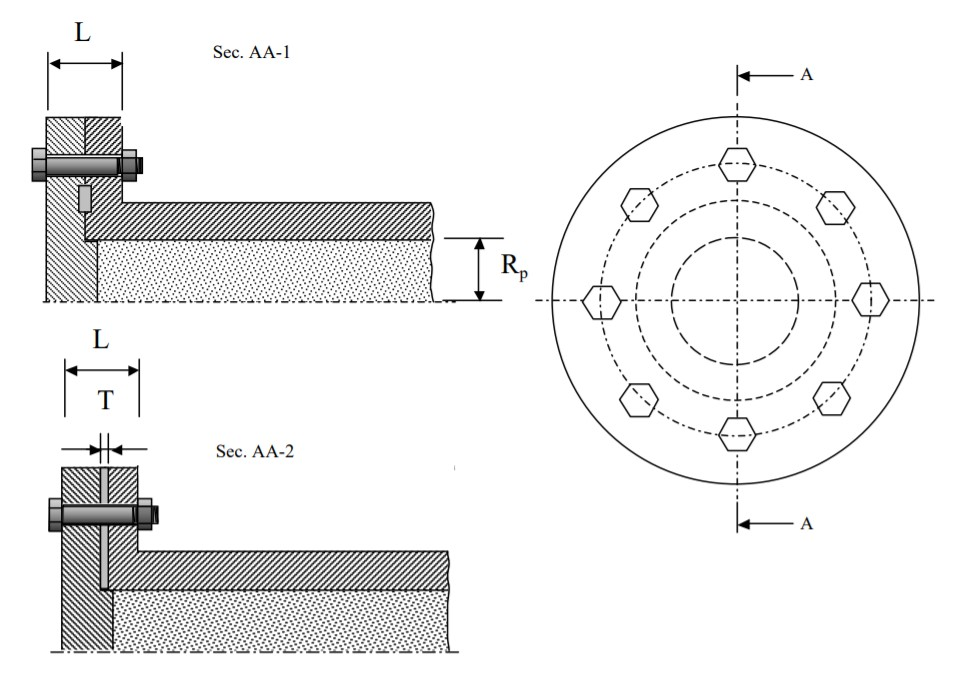
\includegraphics[width=11cm]{gasket}
		\caption{sketch of the cylindrical vessel.} \label{ex:vessel}
	\end{figure}
	
	\paragraph{Problem} A cylindrical vessel (figure \ref{ex:vessel}) is subjected to an internal pressure that varies cyclically between $80bar$ and $250bar$ and is closed by flat ends fastened through 8 equally spaced bolts. Under maximum pressure it is requested to maintain a residual preload of each bolt equal to $N' = 6kN$. 
	
	It is requested to estimate the initial preload necessary for the following design solutions:
	\begin{itemize}
		\item confined gasket;
		\item non-confined gasket.
	\end{itemize}
	In addition it is requested to estimate the fatigue cycle experienced by the bolt in operational conditions and to do its fatigue verification.
	
	Geometrical data known are: the internal radius of the vessel $R_p = 50mm$, the members thickness $t_m=40mm$ ($L$ in figure), the gasket thickness $t_g = 4mm$ ($T$ in the figure) with Young's modulus $E_{rubber} = 1GPa$ and vessel made of steel ($E_{steel} =250 GPa$). The bolts are \texttt{M10 ISO-4014 8.8} with an axial alternate fatigue resistance of $\sigma_{lim,-1} = 420 MPa$ and a notch fatigue factor $K_f = 2.2$.
	
	\paragraph{Solution} The first thing to do is calculate the tensile load acting on each bolt due to the pressure; in particular knowing that the area subjected to such action is $A = \pi R_p^2$, the load that each component will bear is $1/n_b$ of the total (where $n_b = 8$ is the total number of bolts):
	\[ N = \frac{p \pi R_p^2}{n_b} \hspace{2cm} \Rightarrow \qquad N_{max} = 24\,544 N , \quad N_{min} = 7\,854N \]
	
	The next step is to compute the bolt's equivalent stiffness; considering table \ref{tab:bolts} we have that the resisting cross sectional area $A_{bt}$ for a M10 screw is of $58mm^2$, while the cross sectional area of the non-threaded portion can be computed as $A_b = \frac \pi 4 d^2 = 78.54mm^2$. To carry on the analysis we need to define the other parameters of the screw, in particular it's length $l$ can be obtained considering that the screw should at least be long as the sum of the members $t_m$, the nut heigh $m$ (obtained by table \ref{tab:boltsdim}) and at least two pitches $p$:
	\[ l \leq t_f+ m + 2p = 40 +8.4 +2\cdot 1.5 = 51.4mm \]
	Considering that the allowable length series are $45,50,55,\dots mm$ we can chose a screw of $l=55mm$ with threaded portion evaluated as $l_t = 26mm$ (parameter $b$ in table \ref{tab:boltsdim}) and so a non-threaded portion of $l_{nt} = 55- 26 = 29mm$. In the practical case the member thickness $t_m$ is $40mm$, and so the threaded length that subjected to elongation is reduced to $l_t = 11 mm$ (in fact $11+29mm = 40mm$); computing independently the equivalent stiffnesses of the two bids
	\[ K_1 = \frac{E A_{bt}}{l_t} = 1\,107\,273 N/mm \hspace{3cm} K_2 = \frac{E A_{b}}{l_{nt}} = 568\,736 N/mm \]
	then the resulting stiffness obtained as the springs in series become
	\[ K_b = \left(\frac{1}{K_1} + \frac1 {K_2}\right) = 375\, 742 N/mm \]
	
	The study of the equivalent stiffness of the member has instead to be split in 2 cases:
	\begin{itemize}
		\item in the case of a gasket confined in a seat whose effect on the member's stiffness is negligible, it's possible to use the formula of the two truncated conical volumes (equation \ref{eq:conicalstiffness}). In this particular case the members are symmetrical and made of the same material; the equivalent stiffness for each member is so
		\[ K = \frac{\pi E_{steel} d \tan \alpha}{\ln \left( \frac{D_h - d}{D_h+d} \frac{d_0 + d}{d_0-d} \right)} \]
		where parameters are shown in figure \ref{ex:gasketzone}.a are, assuming $\alpha = 30^\circ$ set to: $d_0 = s = 16mm$ obtained by table \ref{tab:boltsdim}, $D_h = d_0 + 2 \frac {t_m} 2 \tan \alpha = 39.09mm$, $d=10mm$. This gives a value $K = 4\,038\,647 N/mm$ and so by considering the two members connected in series gives
		\[ K_{m,cg} = \frac K 2 = 2\,019\, 323 N/mm \]
		\begin{figure}[b!]
			\begin{subfigure}{0.48\linewidth}
				\centering 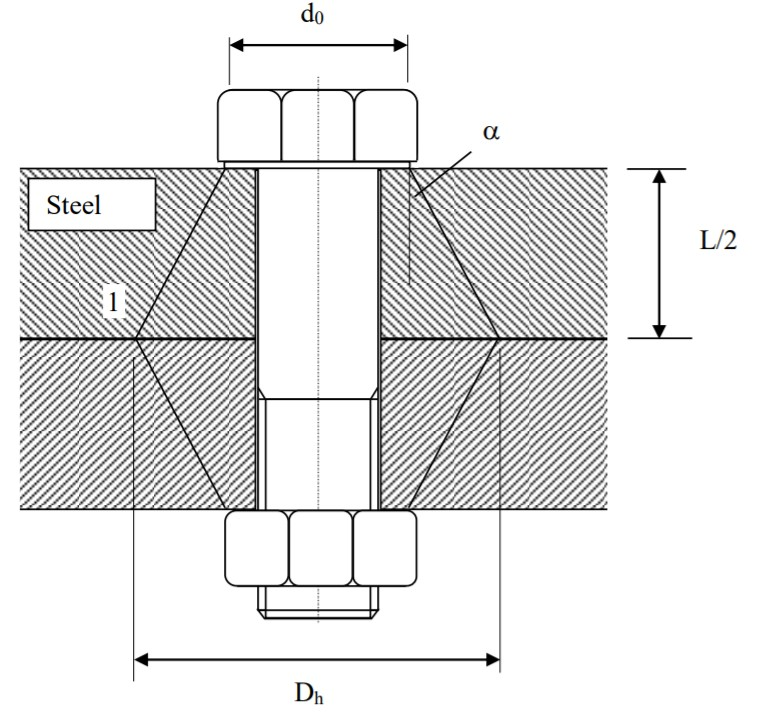
\includegraphics[width=6cm]{gasket-b} \caption{}
			\end{subfigure}
			\begin{subfigure}{0.48\linewidth}
				\centering 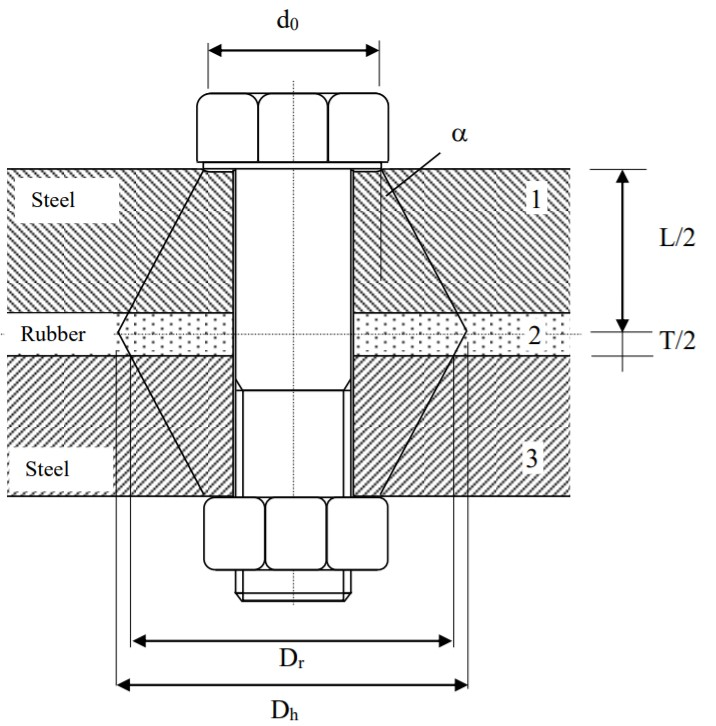
\includegraphics[width=6cm]{gasket-c} \caption{}
			\end{subfigure}
			\caption{ conical stress altered zone due to the compression of the bolt for the confined gasket (a) and not-confined case (b).} \label{ex:gasketzone}
		\end{figure}
		
		\item in the case of non-confined gasket, the rubber material has to be considered while determining the equivalent stiffness of the members; from figure \ref{ex:gasketzone}.b, using geometrical property,  wecan derive $D_r = d_0 + \frac{t_m-t_g}{2} \tan \alpha = 36.78mm$. We so need to compute the stiffnesses $K_s$ of one side of the steel's member and a half of the rubber gasket $K_g$:
		\[ K_s = \frac{\pi E_{steel} d \tan \alpha}{\ln \left( \frac{D_r - d}{D_r+d} \frac{d_0 + d}{d_0-d} \right)} = 525\, 402 N/mm \hspace{2cm} 
		K_g = \frac{\pi E_{rubber} d \tan \alpha}{\ln \left( \frac{D_h - d}{D_h+d} \frac{D_r + d}{D_r-d} \right)} = 131\,350 N/mm \]
		The overall equivalent stiffness of the members for the non confined gasket case is so
		\[ K_{m,ncg} = \frac 12 \left( \frac 1 {K_s} + \frac 1 {K_g}\right)^{-1} = 233\,443 N/mm \]
	\end{itemize}
	With the values of the equivalent stiffnesses  found using equation \ref{eq:boltloadpretension} is possible to determine the portion of external load borne by each bolt:
	\[ N_b = N \frac{K_b}{K_b + K_f} \]
	Substituting the value of the confined gasket gives $N_{b,max,cg} = 3\,850.5N$ and $N_{b,min,cg} = 1\,232N$ while for the non-confined gasket $N_{b,max,ncg} = 15\, 139 N,N_{b,min,cg} = 4\,844N$. Knowing also that, at maximum load condition, the preload on the bolts should be $N' = 6\,000N$, then using 
	\[ N_0 = N' + N_{max} \frac{K_f}{K_b+K_f} \]
	gives the initial preload on the bolt; in particular for the confined gasket case we have $N_{0,cg} = 26\,963.5N$ while for the non-confined one $N_{0,ncg} = 15\,405 N $. Giving the possibility to estimate the elongation $\Delta l_b = N_0/ K_b$ of the bolt and compression $\Delta l_m = - N_0/K_m$ of the members,  then the interference $i = \Delta l_b - \Delta l_f$ can be computed in both cases as
	\[ i_{cg} = 0.071 - (-0.012) = 0.083mm \hspace{3cm} i_{ncg} = 0.041 - (-0.066) = 0.107mm \]
	
	To analyse the fatigue limit it's mandatory to compute the minimum and maximum value of the load cycle whose the bolts are subjected to using equation
	\[ N_{b,max} = N_0 + N_{max} \frac{K_b}{K_b + K_f} \hspace{3cm} N_{b,min} = N_0 + N_{min} \frac{K_b}{K_b + K_f} \]
	resulting in $N_{b,max,cg} = 30\,544N, N_{b,min,cg} = 27\,925N$ for the confined gasket case, while for the non-confined one $N_{b,max,ncg} = 30\,534N, N_{b,min,ncg} = 20\,249N$. Dividing this tension by the  resisting cross sectional area $A_{bt}$ gives the maximum $\sigma_{max} = N_{max}/A_{bt}$ and minimum $\sigma_{min} = N_{min}/A_{bt}$ stress states for the fatigue analysis whose related mean and amplitude value are obtained as
	\[ \sm = \frac{\sigma_{max}+\sigma_{min}}{2} \hspace{3cm} \sa= \frac{\sigma_{max}-\sigma_{min}}{2} \]
	Substituting numerical values gives $\sigma_{m,cg} = 504 MPa, \sigma_{a,cg} = 22.6
	MPa$ for the the confined gasket, $\sigma_{m,ncg} = 437.8 MPa, \sigma_{a,ncg} = 88.7 MPa$ for the non-confined case. To end the fatigue verification is necessary to report the points calculated in the Haigh diagram (figure \ref{ex:gaskethaigh}), paying attention at multiplying only the oscillating term by the notch fatigue factor $K_f = 2.2$. \\	
	As we can see from the diagram, the confined gasket configuration lies in the safe region with safety factor respect to both yield and Goodman line of
	\[ \phi_{ys} = \frac{AC}{AB} = 1.92 \hspace{3cm} \phi_\textrm{Goodman} = \frac{AC'}{AB} = 2.45 \]
	The non-confined gasket configuration lies outside the safe region thus it doesn't pass the fatigue verification.
	
	\begin{SCfigure}[1][b]
		\centering 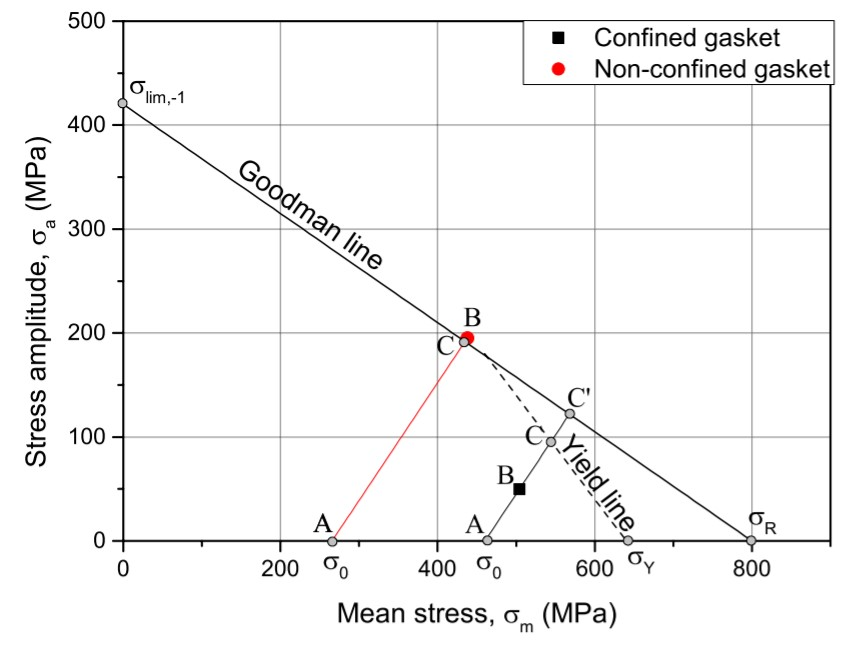
\includegraphics[width=8cm]{gasket-d}
		\caption{Haigh diagram for the confined gasket case and the non-confined one.} \label{ex:gaskethaigh}
	\end{SCfigure}
	
	
	
	
	
	
	
	
	
	
	
	
	
	
	
	